% Paste this entire file into Overleaf main.tex and select pdfLaTeX.
% All figures and references are embedded; no uploads are required.
\documentclass[conference]{IEEEtran}
\usepackage[T1]{fontenc}
\usepackage{amsmath,amssymb,booktabs,array,tikz,pgfplots}
\pgfplotsset{compat=1.18}
\usepackage[hidelinks]{hyperref}
\usepackage{url,balance}
\newcommand{\artifact}[1]{{\footnotesize\nolinkurl{#1}}}
\title{Card Fraud Triage via Gaussian Mixture Density Scoring\\and Denoising Autoencoder Anomaly Detection}
\author{\IEEEauthorblockN{Yashkumar Nimje, Saksham Narotra, Rudra Pratap Singh Choudhary,\\Abhigya Sachdeva, and Somraj Nandi}
\IEEEauthorblockA{Department of Computer Science and Artificial Intelligence\\
Rishihood University, Sonipat, India\\
Advanced Machine Learning and Deep Learning --- Project 26, Phase 2\\
Faculty supervisor: Shobhit Johri}}
\begin{document}
\maketitle
\begin{abstract}
We compare a Gaussian mixture model (GMM) fitted to legitimate transactions with an undercomplete autoencoder trained using a denoising reconstruction objective for card fraud triage. Both models use the same 29 features and chronological ULB dataset partitions. Architecture selection, seed confirmation and decision thresholds use validation data. On 42,560 historical test transactions containing 52 frauds, GMM achieves average precision (AP) of 0.6773 and the autoencoder achieves 0.4867. At 100 reviews, the autoencoder identifies 40 frauds and GMM identifies 38. At 1,000 reviews both identify 41. Frozen validation thresholds expose differences in false-alarm workload. We document experiments, checkpoint selection and artifact provenance. The historical test partition was previously examined during Phase 1, limiting independent-generalization claims.
\end{abstract}
\begin{IEEEkeywords}
fraud triage, anomaly detection, Gaussian mixture model, denoising autoencoder, precision--recall
\end{IEEEkeywords}
\section{Introduction}
Most card transactions are legitimate, but investigators must prioritize the small subset containing fraud. An anomaly score supports a ranked review queue. A decision threshold defines an alert policy whose workload depends on false alarms and missed fraud.

Project 26 tests whether nonlinear reconstruction of legitimate behavior improves on a probabilistic density baseline. Phase 1 established a GMM and completed the AML evaluation. Phase 2 adds a PyTorch autoencoder, compares architecture and corruption settings, confirms performance across seeds, freezes a checkpoint and model-specific thresholds, and evaluates both systems on identical test rows.

We ask how the models compare across the complete precision--recall ranking and how many frauds each recovers at a review capacity or frozen threshold. These questions emphasize different ranking regions. This report presents the implemented comparison with traceable artifacts and explicit operational counts.

\section{Background and Related Work}
A GMM represents a distribution through weighted Gaussian components. Expectation--maximization (EM) alternates responsibility estimation and parameter updates \cite{em}. This gives a likelihood-based model for legitimate transaction behavior. Component count and covariance structure control flexibility and numerical conditioning.

An autoencoder reconstructs an input through a latent representation. Sakurada and Yairi studied reconstruction-based anomaly detection with nonlinear dimensionality reduction \cite{sakurada}. This motivates the hypothesis that transactions departing from learned regularities may have large reconstruction errors. Fraud resembling legitimate transactions may still reconstruct accurately.

Vincent et al.\ developed denoising representation learning through reconstruction of clean inputs from corrupted observations \cite{vincent}. Here, Gaussian noise affects training inputs while targets remain clean. The experiment tests whether corruption regularization improves validation ranking. Reconstruction error itself is an anomaly indicator, without a calibrated interpretation as fraud probability.

The ULB benchmark \cite{dataset} provides anonymized numerical features, elapsed time, transaction amount and a binary fraud label. It supports a common feature and split contract. Anonymization restricts semantic interpretation of individual feature residuals.

\section{Dataset and Experimental Protocol}
\subsection{Source and Chronological Partitions}
The source contains 284,807 transactions, including 492 frauds. Removing 1,081 exact duplicates leaves 283,726 observations with 473 frauds. Table~\ref{tab:splits} records the frozen chronological partitions. Only the 198,242 legitimate training rows enter model fitting.

\begin{table}[!ht]
\caption{Frozen partitions after deduplication}\label{tab:splits}
\centering\small
\begin{tabular}{lrrr}\toprule
Partition & Rows & Legitimate & Fraud\\\midrule
Training & 198,608 & 198,242 & 366\\
Validation & 42,558 & 42,503 & 55\\
Test & 42,560 & 42,508 & 52\\\bottomrule
\end{tabular}
\end{table}

The exact elapsed-time ranges are training up to 132,906 seconds, validation from 132,906 to 151,320 seconds, and test from 151,320 to 172,792 seconds. These ranges share endpoint timestamps because transactions can have identical times. The frozen raw-row-ID rule assigns row 199323 at 132,906 seconds to training and row 199324 to validation. At 151,320 seconds, row 242066 belongs to validation, while rows 242063, 242064 and 242065 belong to test. The frozen ID lists, rather than overlapping inclusive time filters, determine membership.

Membership uses the original zero-based raw row ID. The split manifest records the source checksum and ID lists. Frozen membership resolves transactions sharing boundary timestamps and preserves the Phase 1 partition membership. Score exports retain stable ID, split, model name and anomaly score. Evaluation labels are stored separately and joined one-to-one.

The evidence is \artifact{data/split_manifest.json} and \artifact{data/splits/}. Test prevalence is $52/42560$, approximately $0.1222\%$, which defines the precision--recall prevalence reference.

\subsection{Features and Fitting Boundaries}
Each model receives $V_1,\ldots,V_{28}$ and $\log(1+\mathrm{Amount})$, giving 29 features. Time determines membership and is excluded from inputs. The target \texttt{Class} is excluded from the input matrix. Robust scaling is fitted on legitimate training rows and applied elsewhere without refitting.

GMM uses its frozen Phase 1 scaler and AE its frozen Phase 2 scaler. Final inference verifies that the resulting test feature matrices agree exactly. Thus preprocessing differences do not explain the paired comparison. Feature order and identities appear in \artifact{data/artifacts/feature_metadata.json} and the threshold manifests.

Labels support legitimate-row filtering, validation model selection and evaluation. The protocol therefore uses legitimate-only fitting with labeled validation selection. This requires reliable historical labels for those purposes.

\subsection{Prior Holdout Exposure}
The test partition was examined during Phase 1. Phase 2 uses it as a historical comparison set with known prior exposure. Architecture decisions and threshold calibration use validation data. Models and policies are frozen before the paired test evaluation. No model or threshold adjustment follows the reported test results.

\begin{figure}[!ht]\centering
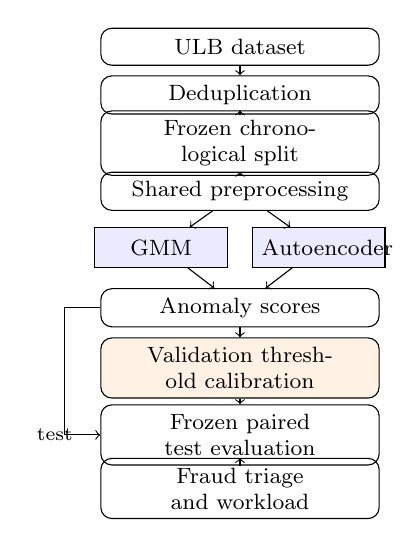
\begin{tikzpicture}[x=1cm,y=.85cm,
every node/.style={font=\footnotesize,align=center},
box/.style={draw,rounded corners,text width=3.3cm,minimum height=.47cm},
model/.style={draw,fill=blue!8,text width=1.45cm,minimum height=.5cm}]
\node[box] (raw) at (0,0) {ULB dataset};
\node[box] (dedup) at (0,-.72) {Deduplication};
\node[box] (split) at (0,-1.44) {Frozen chronological split};
\node[box] (prep) at (0,-2.16) {Shared preprocessing};
\node[model] (gmm) at (-1,-3) {GMM};
\node[model] (ae) at (1,-3) {Autoencoder};
\node[box] (scores) at (0,-3.9) {Anomaly scores};
\node[box,fill=orange!10] (cal) at (0,-4.8) {Validation threshold calibration};
\node[box] (eval) at (0,-5.8) {Frozen paired test evaluation};
\node[box] (triage) at (0,-6.6) {Fraud triage and workload};
\draw[->] (raw)--(dedup);\draw[->] (dedup)--(split);\draw[->] (split)--(prep);
\draw[->] (prep)--(gmm);\draw[->] (prep)--(ae);
\draw[->] (gmm)--(scores);\draw[->] (ae)--(scores);
\draw[->] (scores)--(cal);
\draw[->] (cal)--(eval);
\draw[->] (scores.west) -- ++(-.45,0) |- node[pos=.75,left,font=\scriptsize]{test} (eval.west);
\draw[->] (eval)--(triage);
\end{tikzpicture}
\caption{Overall workflow. Models fit legitimate training rows. Validation scores calibrate thresholds; test scores enter the paired evaluation after the freeze.}
\label{fig:workflow}\end{figure}

\section{Models and Scores}
\subsection{Gaussian Mixture Baseline}
For preprocessed $\mathbf{x}\in\mathbb{R}^{29}$, the density is
\begin{equation}
p(\mathbf{x})=\sum_{k=1}^{K}\pi_k
\mathcal{N}(\mathbf{x};\boldsymbol{\mu}_k,\boldsymbol{\Sigma}_k).
\end{equation}
EM fits parameters on legitimate training transactions. Phase 1 included an AIC/BIC component sweep and covariance experiments. The Phase 2 comparison retains the reproduced saved baseline with 14 full-covariance components, regularization $10^{-6}$, three initializations and seed 42.

Its anomaly score is
\begin{equation}
s_{\mathrm{GMM}}(\mathbf{x})=-\log p(\mathbf{x}).
\end{equation}
Larger scores indicate lower legitimate density. The baseline provenance records validation AP of 0.650975 in \artifact{data/scores/gmm_baseline_provenance.json}. The saved model identity governs this comparison, including where historical notebook runs used other component counts.

\subsection{Implemented Autoencoder}
The frozen dense topology is $29\rightarrow32\rightarrow16\rightarrow32\rightarrow29$. The two 32-unit hidden blocks use batch normalization and LeakyReLU with slope 0.1. The bottleneck and reconstruction layers are linear. Unconstrained output accommodates signed robust-scaled inputs. Figure~\ref{fig:architecture} shows these implemented dimensions.

\begin{figure}[!ht]\centering
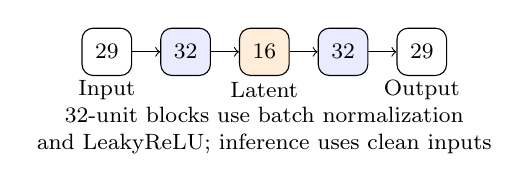
\begin{tikzpicture}[x=.8cm,y=.8cm,every node/.style={font=\footnotesize},
box/.style={draw,rounded corners,minimum width=.63cm,minimum height=.6cm}]
\node[box] (a) at (0,0) {29};
\node[box,fill=blue!8] (b) at (1.25,0) {32};
\node[box,fill=orange!15] (c) at (2.5,0) {16};
\node[box,fill=blue!8] (d) at (3.75,0) {32};
\node[box] (e) at (5,0) {29};
\draw[->] (a)--(b);\draw[->] (b)--(c);\draw[->] (c)--(d);\draw[->] (d)--(e);
\node at (0,-.6) {Input};\node at (2.5,-.6) {Latent};\node at (5,-.6) {Output};
\node[align=center] at (2.5,-1.25) {32-unit blocks use batch normalization\\and LeakyReLU; inference uses clean inputs};
\end{tikzpicture}
\caption{Frozen AE. Training inputs receive corruption and targets stay clean.}\label{fig:architecture}
\end{figure}

With encoder $f_\theta$ and decoder $g_\phi$, training minimizes
\begin{equation}
\mathcal{L}=\frac{1}{N}\sum_{i=1}^{N}\frac{1}{29}
\left\|\mathbf{x}_i-g_\phi(f_\theta(\widetilde{\mathbf{x}}_i))\right\|_2^2.
\end{equation}
The selected denoising configuration uses
$\widetilde{\mathbf{x}}=\mathbf{x}+\boldsymbol{\epsilon}$ with
$\boldsymbol{\epsilon}\sim\mathcal{N}(0,0.5^2 I)$. Clean variants use $\widetilde{\mathbf{x}}=\mathbf{x}$. All training examples are legitimate.

Inference disables corruption and computes
\begin{equation}
s_{\mathrm{AE}}(\mathbf{x})=\frac{1}{29}
\left\|\mathbf{x}-g_\phi(f_\theta(\mathbf{x}))\right\|_2^2.
\end{equation}
The checkpoint is loaded into evaluation mode with gradients disabled. Higher error ranks a transaction as more anomalous. The implementation and frozen manifest determine the reported architecture, correcting an earlier draft methods diagram.

\section{Experiments and Selection}
\subsection{Training and Regularization}
The ablations use Adam at learning rate $0.001$, batch size 256, zero weight decay and at most 100 epochs. Early stopping monitors legitimate-validation reconstruction MSE with patience 10. The best validation-loss weights are restored. Validation AP compares configurations. Both checkpoint and configuration decisions use validation data.

The realized settings follow Addendum A1 of \artifact{docs/ae_experiment_plan.md}. In particular, noise standard deviation is 0.5 in scaled units. Saved run settings supersede preliminary planning suggestions about other noise levels or activations.

\subsection{Architecture and Denoising Ablations}
Stage 1 compares clean bottleneck widths 4, 8 and 16 at seed 42, then denoising at the best clean width. Table~\ref{tab:ablation} transcribes \artifact{results/phase2/ae_run_log.csv}. Width 16 gives the strongest clean validation AP. Denoising at this width raises AP from 0.198333 to 0.340914.

\begin{table}[!ht]
\caption{Stage 1 validation results, seed 42}\label{tab:ablation}
\centering\small
\begin{tabular}{lrrr}\toprule
Configuration & AP & Prec.@100 & Best epoch\\\midrule
4, clean & .075492 & .02 & 57\\
8, clean & .131272 & .21 & 99\\
16, clean & .198333 & .32 & 37\\
16, denoising & .340914 & .39 & 99\\\bottomrule
\end{tabular}
\end{table}

The experiment varies width and corruption while retaining the declared backbone and training budget. Lower reconstruction loss alone need not improve fraud ranking because legitimate and fraudulent reconstruction errors can overlap.

\subsection{Seed Confirmation}
Stage 2 compares width-16 denoising and the width-8 clean reference across seeds 0, 7 and 42, reusing Stage 1 seed-42 runs. Table~\ref{tab:seed} gives AP and sample standard deviation across three seeds, as recorded in the run log and \artifact{results/ae_seed_stability.md}.

\begin{table}[!ht]
\caption{Validation AP across confirmation seeds}\label{tab:seed}
\centering\footnotesize
\begin{tabular}{lrrr}\toprule
Seed & 8, clean & 16, denoising\\\midrule
0 & .205460 & .311635\\
7 & .177996 & .324527\\
42 & .131272 & .340914\\\midrule
Mean & .171576 & .325692\\
Sample SD & .037512 & .014674\\\bottomrule
\end{tabular}
\end{table}

The final configuration is selected by mean validation AP. The checkpoint is selected by the seed whose AP is closest to that mean. Seed 7 is closest for width-16 denoising, producing \texttt{RUN-S2-W16-DNZ-S7} with validation AP 0.324527. Its hash and settings are frozen in \artifact{results/ae_frozen_model_manifest.json}. This policy avoids selecting only the largest individual AP.

\section{Evaluation and Threshold Freezing}
\subsection{Ranking and Review Metrics}
Average precision is the primary ranking summary,
\begin{equation}
\mathrm{AP}=\sum_n(R_n-R_{n-1})P_n.
\end{equation}
The shared evaluation utility implements this definition. AP is primary because precision directly measures the fraction of alerts that are genuine frauds. With only about 0.122\% fraud prevalence on test, even a small false-positive rate can produce many false alarms. ROC-AUC measures ranking over true-positive and false-positive rates; its large legitimate denominator can make those operational counts less apparent. Reporting AP and the PR curve emphasizes fraud recovery together with alert quality. AP is prevalence-dependent, so comparisons here use identical test membership. ROC-AUC remains a secondary measure, complemented by explicit capacity and threshold tables. At capacity $K$, precision is the fraction of frauds in the $K$ highest scores and recall is the caught fraction of all frauds. Equal-score top-$K$ ordering uses lexical stable row ID for both models, ensuring consistency under CSV row permutations.

\subsection{Validation-Only Policies}
For $\alpha\in\{0.001,0.01,0.05\}$, the existing selector maximizes validation recall subject to validation FPR $\leq\alpha$. When recall ties, it retains the highest threshold. A transaction is flagged if $s(\mathbf{x})\geq\tau$, including all members of a tied-score group.

Table~\ref{tab:freeze} records both freezes. Actual validation FPR can be below budget because the rule avoids extra alerts without recall gain. The values remain fixed during test reporting. Unsupported operating points have explicit no-alert or undefined statuses in the schema. All six reported policies have status \texttt{ok}.

\begin{table}[!ht]
\caption{Frozen validation policies}\label{tab:freeze}
\centering\small
\begin{tabular}{llrrr}\toprule
Model & Budget & Threshold & Recall \% & FPR \%\\\midrule
GMM & 0.1\% & 143.650819 & 76.36 & .0212\\
GMM & 1\% & 67.959492 & 80.00 & .2376\\
GMM & 5\% & 39.182022 & 87.27 & 3.2468\\
AE & 0.1\% & 4.156134 & 47.27 & .0823\\
AE & 1\% & .889055 & 80.00 & .8423\\
AE & 5\% & .458263 & 83.64 & 2.7292\\\bottomrule
\end{tabular}
\end{table}

Full-precision values, score transforms, hashes and feature identities appear in the GMM and AE \artifact{results/phase2/} threshold manifests. Score magnitudes from different model families have different meanings. Independent calibration permits operational comparisons without treating their raw values as equivalent.

\begin{table*}[t]
\caption{Test behavior at validation-selected thresholds. Budget refers to validation FPR.}
\label{tab:testpolicy}\centering\small
\begin{tabular}{llrrrrrrr}\toprule
Model & Budget & Alerts & Caught & Missed & False alarms & Test recall \% & Test FPR \% & Test precision \%\\\midrule
GMM & 0.1\% & 37 & 33 & 19 & 4 & 63.46 & .0094 & 89.19\\
AE & 0.1\% & 38 & 24 & 28 & 14 & 46.15 & .0329 & 63.16\\
GMM & 1\% & 107 & 38 & 14 & 69 & 73.08 & .1623 & 35.51\\
AE & 1\% & 241 & 40 & 12 & 201 & 76.92 & .4729 & 16.60\\
GMM & 5\% & 955 & 41 & 11 & 914 & 78.85 & 2.1502 & 4.29\\
AE & 5\% & 808 & 41 & 11 & 767 & 78.85 & 1.8044 & 5.07\\\bottomrule
\end{tabular}
\end{table*}
\section{Final Paired Results}
\subsection{Ranking Performance}
On identical test rows, GMM achieves AP 0.677302 and ROC-AUC 0.906694. AE achieves AP 0.486678 and ROC-AUC 0.919871. Thus GMM has higher AP while the secondary ROC summary favors AE. Figure~\ref{fig:pr} shows the empirical PR curves and prevalence baseline.

\begin{figure}[!ht]\centering
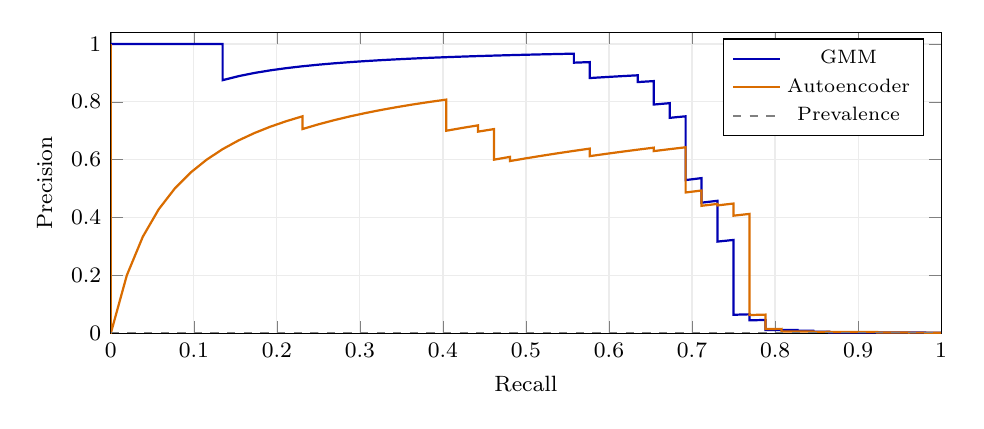
\begin{tikzpicture}
\begin{axis}[width=\columnwidth,height=5.4cm,
xlabel=Recall,ylabel=Precision,xmin=0,xmax=1,ymin=0,ymax=1.04,
tick label style={font=\footnotesize},label style={font=\footnotesize},
legend style={font=\scriptsize,at={(.98,.98)},anchor=north east},
grid=major,grid style={gray!15}]
\addplot[color=blue!70!black,thick] coordinates {(1,0.001221804511) (1,0.001404797925) (0.9807692308,0.001377819803) (0.9807692308,0.00192278691) (0.9615384615,0.001885156279) (0.9615384615,0.002032437706) (0.9423076923,0.001991869919) (0.9423076923,0.001999755132) (0.9230769231,0.001959023753) (0.9230769231,0.002038389672) (0.9038461538,0.001996007984) (0.9038461538,0.002007174581) (0.8846153846,0.001964552637) (0.8846153846,0.001965056175) (0.8653846154,0.001922419686) (0.8653846154,0.004931506849) (0.8461538462,0.004822446295) (0.8461538462,0.008387342737) (0.8269230769,0.00819828408) (0.8269230769,0.01104546622) (0.8076923077,0.01079136691) (0.8076923077,0.0109832636) (0.7884615385,0.01072456186) (0.7884615385,0.04545454545) (0.7692307692,0.04439511654) (0.7692307692,0.06504065041) (0.75,0.06351791531) (0.75,0.3223140496) (0.7307692308,0.3166666667) (0.7307692308,0.4578313253) (0.7115384615,0.4512195122) (0.7115384615,0.5362318841) (0.6923076923,0.5294117647) (0.6923076923,0.75) (0.6730769231,0.7446808511) (0.6730769231,0.7954545455) (0.6538461538,0.7906976744) (0.6538461538,0.8717948718) (0.6346153846,0.8684210526) (0.6346153846,0.8918918919) (0.6153846154,0.8888888889) (0.5961538462,0.8857142857) (0.5769230769,0.8823529412) (0.5769230769,0.9375) (0.5576923077,0.935483871) (0.5576923077,0.9666666667) (0.5384615385,0.9655172414) (0.5192307692,0.9642857143) (0.5,0.962962963) (0.4807692308,0.9615384615) (0.4615384615,0.96) (0.4423076923,0.9583333333) (0.4230769231,0.9565217391) (0.4038461538,0.9545454545) (0.3846153846,0.9523809524) (0.3653846154,0.95) (0.3461538462,0.9473684211) (0.3269230769,0.9444444444) (0.3076923077,0.9411764706) (0.2884615385,0.9375) (0.2692307692,0.9333333333) (0.25,0.9285714286) (0.2307692308,0.9230769231) (0.2115384615,0.9166666667) (0.1923076923,0.9090909091) (0.1730769231,0.9) (0.1538461538,0.8888888889) (0.1346153846,0.875) (0.1346153846,1) (0.1153846154,1) (0.09615384615,1) (0.07692307692,1) (0.05769230769,1) (0.03846153846,1) (0.01923076923,1) (0,1)};
\addlegendentry{GMM}
\addplot[color=orange!85!black,thick] coordinates {(1,0.001221804511) (1,0.001505370118) (0.9807692308,0.001476463436) (0.9807692308,0.001709344416) (0.9615384615,0.001675884029) (0.9615384615,0.0018972452) (0.9423076923,0.00185937085) (0.9423076923,0.002183795347) (0.9230769231,0.002139323439) (0.9230769231,0.003885381253) (0.9038461538,0.003804743787) (0.9038461538,0.003998298596) (0.8846153846,0.003913561341) (0.8846153846,0.004247068599) (0.8653846154,0.004155124654) (0.8653846154,0.004414361389) (0.8461538462,0.004316687923) (0.8461538462,0.005409392673) (0.8269230769,0.00528710193) (0.8269230769,0.005952380952) (0.8076923077,0.005814758411) (0.8076923077,0.01475755446) (0.7884615385,0.0144112478) (0.7884615385,0.0640625) (0.7692307692,0.06259780908) (0.7692307692,0.412371134) (0.75,0.40625) (0.75,0.4482758621) (0.7307692308,0.4418604651) (0.7307692308,0.4470588235) (0.7115384615,0.4404761905) (0.7115384615,0.4933333333) (0.6923076923,0.4864864865) (0.6923076923,0.6428571429) (0.6730769231,0.6363636364) (0.6538461538,0.6296296296) (0.6538461538,0.641509434) (0.6346153846,0.6346153846) (0.6153846154,0.6274509804) (0.5961538462,0.62) (0.5769230769,0.612244898) (0.5769230769,0.6382978723) (0.5576923077,0.6304347826) (0.5384615385,0.6222222222) (0.5192307692,0.6136363636) (0.5,0.6046511628) (0.4807692308,0.5952380952) (0.4807692308,0.6097560976) (0.4615384615,0.6) (0.4615384615,0.7058823529) (0.4423076923,0.696969697) (0.4423076923,0.71875) (0.4230769231,0.7096774194) (0.4038461538,0.7) (0.4038461538,0.8076923077) (0.3846153846,0.8) (0.3653846154,0.7916666667) (0.3461538462,0.7826086957) (0.3269230769,0.7727272727) (0.3076923077,0.7619047619) (0.2884615385,0.75) (0.2692307692,0.7368421053) (0.25,0.7222222222) (0.2307692308,0.7058823529) (0.2307692308,0.75) (0.2115384615,0.7333333333) (0.1923076923,0.7142857143) (0.1730769231,0.6923076923) (0.1538461538,0.6666666667) (0.1346153846,0.6363636364) (0.1153846154,0.6) (0.09615384615,0.5555555556) (0.07692307692,0.5) (0.05769230769,0.4285714286) (0.03846153846,0.3333333333) (0.01923076923,0.2) (0,0) (0,1)};
\addlegendentry{Autoencoder}
\addplot[gray,dashed,domain=0:1] {0.0012218045112781955};
\addlegendentry{Prevalence}
\end{axis}\end{tikzpicture}
\caption{Test precision--recall curves derived from the committed scores. AP is computed separately using the shared evaluation function.}
\label{fig:pr}\end{figure}

The evidence is \artifact{results/phase2/paired/ranking.csv} and the two test score exports. This report uses the verified GMM export rather than inconsistent historical report values. Fresh GMM inference agrees with the export within maximum absolute difference $2.85\times10^{-14}$.

\subsection{Fixed Review Capacity}
Table~\ref{tab:capacity} shows capacity-specific recovery. At 100 reviews GMM catches 38 frauds with 62 false alarms, while AE catches 40 with 60. All 38 GMM catches are shared. The two AE-only frauds have raw IDs 272521 and 274475. At 500 reviews there are 39 shared frauds and one additional AE catch. At 1,000 reviews the models catch the same 41 frauds, each with 959 false alarms.

\begin{table}[!ht]
\caption{Fixed-capacity test triage}\label{tab:capacity}
\centering\small
\begin{tabular}{llrrrr}\toprule
Model & $K$ & Caught & Recall \% & Prec.\ \% & FP\\\midrule
GMM & 100 & 38 & 73.08 & 38.00 & 62\\
AE & 100 & 40 & 76.92 & 40.00 & 60\\
GMM & 500 & 39 & 75.00 & 7.80 & 461\\
AE & 500 & 40 & 76.92 & 8.00 & 460\\
GMM & 1,000 & 41 & 78.85 & 4.10 & 959\\
AE & 1,000 & 41 & 78.85 & 4.10 & 959\\\bottomrule
\end{tabular}
\end{table}

The sources are \artifact{results/phase2/paired/triage.csv} and \artifact{results/phase2/paired/overlap.csv}. The two-case difference describes this queue; a multi-period study would be needed to characterize its reliability.

\subsection{Frozen Thresholds and Workload}
Table~\ref{tab:testpolicy} applies the saved validation policies to test scores. At the strictest budget, GMM catches 33 frauds with four false alarms; AE catches 24 with 14. At the 1\% budget AE catches two extra frauds with 132 extra false alarms. At the 5\% budget both catch 41, with fewer false alarms for AE.



The source is \artifact{results/phase2/paired/thresholds.csv}. A validation FPR budget does not guarantee the same realized FPR on later transactions. The models also produce different alert counts at the same budget, so the false-alarm and workload counts must accompany recall. Capacity tables instead hold reviews fixed.

\section{Reproducibility and Evidence}
Final inference reloads the selected checkpoint and frozen preprocessing and verifies raw data against the split checksum. Shared-contract checks reject missing or duplicated IDs, wrong splits, non-finite scores and incomplete label joins. The receipt links scores to model, scaler, policy and code identities. Test feature matrices agree exactly.

The committed inference environment uses Python 3.12.14, PyTorch 2.8.0, NumPy 2.0.2, pandas 2.3.3, scikit-learn 1.6.1 and joblib 1.5.3. The inference receipt and evaluation provenance in \artifact{results/phase2/paired/} record these versions and the corresponding code and input identities.

Reproduction runs frozen test inference followed by the paired evaluation script. Exact commands appear in \artifact{docs/paired_evaluation.md}. The freeze scripts also verify saved policies against validation-only recalibration.

For this report revision, running \texttt{python -m pytest -q} with the pinned data dependencies produced 105 passes, three skips and one failure. The exact command, package versions and output are committed in \artifact{reports/phase2/full_suite_test_log.txt}. The skipped historical AE tests require an absent run directory. The failure is an inference-code identity check after the later workflow integration changed \artifact{src/models/autoencoder.py}, while the paired inference receipt still records the earlier code hash. This failure prevents a fully passing full-suite claim. It does not indicate a changed score export; the report's numerical tables remain tied to the committed paired artifacts at snapshot \texttt{252197f}. The earlier 98-pass summary is superseded here by the reproducible current run. Data-layer verification and dependencies appear in \artifact{docs/Phase2_Data_Reproducibility.md} and \artifact{requirements-data.txt}.

\section{Discussion and Limitations}
\subsection{Metric-Dependent Trade-offs}
Higher GMM AP and higher AE precision at 100 reviews are compatible. AP summarizes precision across recall increments, whereas a fixed queue examines one operating region. AE includes two extra frauds in that queue but yields lower AP across the overall ranking. A triage policy therefore needs an explicit capacity or false-positive constraint.

Denoising improves validation AP relative to the clean width-16 model. This supports the selected setting among attempted configurations. It does not establish that every noise level helps or that reconstruction universally improves on density estimation. GMM remains stronger on AP in this study.

\subsection{Scope and Uncertainty}
Only 52 frauds occur in test, so one case moves recall by approximately 1.92 percentage points. The three-seed study measures validation variability, without providing a confidence interval for future deployment performance.

The dataset spans a short historical period and anonymizes most features. No independent external dataset validation has been performed. No customer-level grouping analysis was conducted, and the anonymized features do not establish account-level separation across partitions. New fraud mechanisms and long-term drift therefore remain untested. Deduplication and chronological membership support reproducibility, while production readiness needs separate operational evidence.

Frauds resembling legitimate behavior can reconstruct accurately. GMM quality depends on component adequacy and numerical conditioning. Both models miss 11 frauds at 1,000 reviews. Real-world analyst review costs have not been measured. Customer friction and lost monetary value are unquantified because verified cost inputs are absent. No production deployment or online monitoring evaluation has been performed.

The test partition had prior Phase 1 exposure. This report discloses that exposure while preserving Phase 2 validation-only selection and the frozen comparison. Independent confirmation requires a fresh time period.

\subsection{Deferred Work}
Standalone GMM and AE comparison is complete. Score fusion, latent-space density models, supervised fine-tuning, online updating, deployment and autonomous blocking remain deferred. Hybrid or production-benefit claims require additional experiments.

\section{Member Contributions}
Yashkumar Nimje led frozen data provenance and split coordination, experiment orchestration and AE threshold calibration. Saksham Narotra implemented shared preprocessing, loaders, corruption handling and data-pipeline reproducibility checks. Rudra Pratap Singh Choudhary implemented GMM reproduction, reference AE and inference, and contributed methodology. Abhigya Sachdeva designed experiments, ran ablations, analyzed seed stability, selected the checkpoint and documented the model card. Somraj Nandi implemented the shared evaluation contract, GMM freeze, final paired evaluation and technical report assembly. The repository issues and committed artifacts trace these responsibilities \cite{repo}.

\section{Practical Interpretation}
For a team emphasizing performance across the complete ranking, the verified results favor GMM on AP. For a fixed 100-case review queue on this test period, AE recovers two additional frauds while generating two fewer false alarms. At the strictest frozen validation budget, GMM catches more fraud with fewer false alarms. Threshold-based workloads differ substantially at the other budgets as well. Preference should therefore depend on the declared review capacity and acceptable workload, with both models assessed on future independent data before operational adoption. Neither model is universally superior across the measured criteria.

\section{Conclusion}
This paired experiment demonstrates an operating-point trade-off. GMM achieves AP 0.6773, while the denoising AE achieves 0.4867 and catches two extra frauds in 100 reviews. At 1,000 reviews both recover 41 frauds. Frozen policies quantify false-alarm workloads. Scores, manifests and logs provide reproducible evidence within the stated historical-data limitations.

\balance
\begin{thebibliography}{00}
\bibitem{em} A. P. Dempster, N. M. Laird, and D. B. Rubin, Maximum likelihood from incomplete data via the EM algorithm, \emph{J. Royal Stat. Soc., Series B}, vol. 39, no. 1, pp. 1--38, 1977. doi: 10.1111/j.2517-6161.1977.tb01600.x.
\bibitem{sakurada} M. Sakurada and T. Yairi, Anomaly detection using autoencoders with nonlinear dimensionality reduction, in \emph{Proc. MLSDA}, 2014, pp. 4--11. doi: 10.1145/2689746.2689747.
\bibitem{vincent} P. Vincent, H. Larochelle, Y. Bengio, and P.-A. Manzagol, Extracting and composing robust features with denoising autoencoders, in \emph{Proc. ICML}, 2008, pp. 1096--1103. doi: 10.1145/1390156.1390294.
\bibitem{dataset} ULB Machine Learning Group, Credit card fraud detection, Kaggle. [Online]. \url{https://www.kaggle.com/datasets/mlg-ulb/creditcardfraud}. Accessed Nov. 17, 2026.
\bibitem{repo} Project 26 team, Card-Fraud-Triage-ML-DL, source snapshot \texttt{252197f}, 2026. [Online]. \url{https://github.com/WizardCarp85/Card-Fraud-Triage-ML-DL}.
\end{thebibliography}
\end{document}
